\documentclass[12pt]{article}

\usepackage[utf8]{inputenc}
\usepackage[T1]{fontenc}
\usepackage{geometry}
\usepackage{graphicx} %figures
\usepackage{subfig} %subfigures
\usepackage{gensymb} %degree sign
\usepackage{amsmath} %math stuff
\usepackage{bm} %bold stuff
\usepackage[]{algorithm2e} %algorithms
\geometry{a4paper}

\title{\textbf{Part 12: Multi-Fidelity Gaussian Processes}}

\begin{document}
\date{February 15, 2021}
\maketitle

This should hopefully be an interesting post. We will be talking about using Gaussian Processes (GPs) for modeling with multiple data sources, or fidelities. For example, what is the true concentration of a pollutant if we have multiple measurements from different devices, given that said devices may have different biases,  variances, locations, and costs of operation?

\section{The Multi-Fidelity GP Model}

Let us utilize fidelity levels $l$. We wish to model a true underlying process $f_0(x) \sim GP(0,K_0)$. We will utilize multiple fidelities $f_l(x) = g(x) + \delta_l(x)$ with a GP model of the deviance from the true process $\delta_l(x) \sim GP(0,K_l)$. The underlying process $l=0$ can have a squared exponential covariance kernel:

\begin{align*}
K_0(x,x') = \sigma_f^2exp(-0.5\Sigma_i^p\dfrac{(x_{i}-x'_{i})^2}{\lambda_{i}})
\end{align*}

\vspace{5mm}

Which means the underlying process has $p+2$ hyperparameters. Due to $f_l(x) = g(x) + \delta_l(x)$ being the model of the fidelities $l>0$, each process $l$ will have it's own squared exponential kernel plus the underlying kernel:

\begin{align*}
K_l(x,x') = K_0(x,x') + \sigma_f^2exp(-0.5\Sigma_i^p\dfrac{(x_{i}-x'_{i})^2}{\lambda_{i}})
\end{align*}

\vspace{5mm}

We are also going to assume fidelity independence, which means $K_l(x,x')$ will be calculated as above only when $l=l'$ for $x$ and $x'$. If $l \neq l'$ or $l=0$ (as stated above) then $K_l(x,x') = K_0(x,x')$. So (as in the code attached) when calculating the kernel matrix just use a bunch of \emph{if} statements to construct the kernel based on the identity of the data $x$ and $x'$.

\vspace{5mm}

To calculate mean and standard deviation:

\begin{equation}
\mu(x^*) = K(x^*,X)(K(X,X)+sI)^{-1}Y
\end{equation}

\begin{equation}
\sigma^2(x^*) = K(x^*,x^*)-K(x^*,X)(K(X,X)+sI)^{-1}K(X,x^*)
\end{equation}

\vspace{5mm}

Where $s$ is a vector of $\sigma^2(X)$ hyperparameters.

\section{Hyperparameter Optimization}

Here we will optimize the standard likelihood function (log) using L-BFGS-B implemented in \emph{sci-py}. I will spare you the gory details, and I'm not 100\% sure I'm correct in the calculation of my gradient, but below is a plot of some random data with the following functional form:

\begin{align*}
f_0(x)=-X_1 + U(-10^{-2},10^{-2})
\end{align*}

\begin{align*}
f_1(x)=-X_1 + U(-10^{-1},10^{-1})
\end{align*}

\vspace{5mm}

Where we will (i) only use $X_1$ in $f(x)$ for simplicity and where if the experiment has a 0 in it's first column it'll be assigned to $f_0(x)$ and if it has a 1 in the first column it'll be assigned to $f_1(x)$. To help, I will bifurcate the data such that we have equally space data points in $X_1$ and one data set will sit on the right side of $X_1$'s design space and the other will occupy the remaining left side. 

\begin{figure}[h]
\centering
\subfloat[][L-BFGS-B \emph{sci-py}]{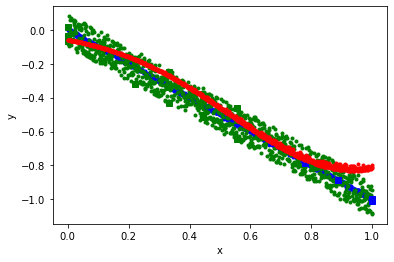
\includegraphics[width=0.4\textwidth]{Post_12_fig1}}
\subfloat[][Botorch]{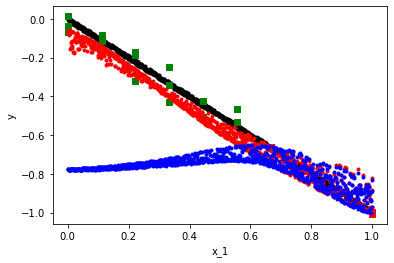
\includegraphics[width=0.4\textwidth]{Post_12_fig2}}
\caption{Multi-Fidelity GP | \textbf{left} my implementation in python (see code) for prediction of $f_0(x)$ in red \textbf{right} Botorch implementation in python for prediction of $f_0(x)$ in red, regular GP using only 0th data in blue, for both plots blue and green squares are the $l=1$ and $l=0$ fidelity data respectively}
\end{figure}

\vspace{5mm}

As you can see both implementations successfully recapitulated the noisy linear trend in red, while Botorch's regular GP (only having access to the highest fidelity model $l=0$ did not do as good. Of course what is the value in this? As I said in the top of the post, if we have multiple types of sensors attempting to measure the same thing, we can statistically fuse their data across quality $l$ and space $x$. So our toy problem might represent a type of sensor that is common in one area and not in another. 

\vspace{5mm}

An important thing to note here is that we have treated our problem $f_0(X)$ as being a measure of the true underlying value (or at least the closest we can get) while $f_1(x)$ was merely an approximation. This hierarchy need not be the case as we can predict whatever fidelity we wish by changing the first column in our data $l$. There are other models that treat all information sources equally (rather than being deviations from an underlying process) and we may discuss them in future. 

\vspace{5mm}

Until then we are done! This week was a real fun one but quite difficult. I'll try to do something lighter for next week but haven't decided. See ya!

\end{document}